\documentclass[12pt]{article}
\title{A Decentralized Mnemonic Backup System}
\author{PriFi Labs Inc.}

\date{}

\usepackage{hyperref}
\usepackage{graphicx}


\usepackage{amsmath,proof,amsthm,amssymb}

\usepackage{setspace}
\usepackage{etoolbox}
\AtBeginEnvironment{quote}{\par\singlespacing\small}

\usepackage{enumitem}

\newcommand{\ms}[1]{\ensuremath{\mathsf{#1}}}
\newcommand{\msi}[1]{\ensuremath{\mathsfit{#1}}}

\newcommand{\tx}[3]{\ms{#1}(#3)}
\newcommand{\qry}[3]{\ms{#1}(#3)}

\begin{document}

\maketitle

% \begin{abstract}
%
% \end{abstract}

\section{Introduction}

\begin{quote}
{\em ``Not Your Keys, not Your Coins.''}
\end{quote}

This crypto mantra, popularized by {\em Andreas Antonopoulos}, encourages us, crypto enthusiasts, to use non-custodial crypto wallets in which the private keys are directly stored on their device. However, using non-custodial wallets comes with the risk of losing all of our crypto assets if we lose our private keys. If our device gets lost, stolen or irremediably break down, our crypto assets might be locked forever \cite{LostPasswords}.\\

Fortunately, most non-custodial wallets such as Exodus (Bitcoin), Metamask (Ethereum) and Keplr (Secret Network) offer a way to recover our private keys by the mean of a ``recovery phrase'' also known as ``mnemonic seed phrase''. It is the 12-word phrase that we are being given the first time we setup our wallet. Here is an example of such a phrase: 

\begin{quote}
\begin{center}
{\tt witch fox practice feed shame open}\\
{\tt despair creek road again ice least}
\end{center}
\end{quote}

That phrase is important as it is used to generate the same private keys on demand (BIP39 standard \cite{BIP39}). We can use them as a backup or to import our wallet into a new device. Indeed, this mnemonic phrase is a really sensitive piece of information. Anyone who has access to this phrase would have full control over our crypto assets as explained in the [Metamask FAQ page]\cite{MetamaskFAQ}:

\begin{quote}
{\em ``MetaMask requires that you store your Secret Recovery Phrase in a safe place. It is the only way to recover your funds should your device crash or your browser reset. We recommend you to write it down. The most common method is to write your 12-word phrase on a piece of paper and store it safely in a place where only you have access. Note: if you lose your Secret Recovery Phrase, MetaMask can’t help you recover your wallet. Never give you Secret Recovery Phrase or your private key(s) to anyone or any site, unless you want them to have full control over your funds.''}\\
\end{quote}

As written here, we are not supposed to remember that phrase like a password. Instead, it is recommended to write it down on a piece of paper and store it in a ``safe place''. But where is that ``safe place'' exactly? In our physical wallet with our cash and credit cards? Not ideal as it could get lost or stolen. Inside our home? No ideal again as it could burn down. A safe deposit box in the vault of a bank? it might be the best solution after all but the logistics that comes with it makes that solution very cumbersome. \\
 
In the end, it is quite inconvenient to store physical objects safely. So, could we design a simple application that would take custody of my passphrase and would allow me to recover by simply using my email? Yes we could build such an application, it would be something similar to a password manager such as {\em 1password} \cite{1password} for instance. However, such a solution requires 1) that the service provider is trustworthy an 2) that the whole application is secured. Indeed, such a centralized solution is not a good solution as it goes against the philosophy of decentralized application. \\

In this paper, we propose a Decentralized Mnemonic Backup system that anyone can use to give custody to any blockchain passphrase to the Secret Network \cite{SecretNetwork} and recover it using a simple email. To better explain our idea, we will go through 3 iterations each more secure than the previous one. The first iteration (section \ref{iteration1}) is meant to be simple to capture the user experience however that first design is rather naive and not very secured. In the second iteration (section \ref{iteration2}), we harden the security by encrypting the passphrase and separating the key management from the passphrase storage. That second iteration makes use of the well know Diffie–Hellman key exchange protocol to securely generate the encryption key on the blockchain. Finally in the last iteration (section \ref{iteration3}), we will split and distributed the encrypted passphrase across the network by using another cryptographic protocol called the Shamir's Secret Sharing scheme. 

\section{Iteration 1: The User Experience}
\label{iteration1}

Alice is a crypto enthusiast that holds all kind of crypto assets: BTC, ETH, SCRT and others. She would like to have an online backup of all of her wallets' passphrases in case her device gets lost, stolen or irremediably breaks down. When that doomsday comes, she should be able to recover her passphrases easily. The overall user experience is rather simple: 

\begin{itemize}
    \item {\bf When Alice wants to backup a passphrase}, she visits our Mnemonic Backup website and enters a passphrase and her email. After submitting her information, our application sends her an email with a confirmation code that she should enter to finalize the backup process. 
    \item {\bf When Alice wants to recover a passphrase}, she visits our Mnemonic Backup website and enters her email. Our application sends her an email with a verification code that she should enter before getting her passphrase back. 
\end{itemize}

This user experience is similar to existing security mechanisms used in traditional web applications where we must make sure that the user is the legitimate owner of the email address used for signing up, signing in (with two factor authentication) or reseting a password.

\subsection{Architecture}

Our Mnemonic Backup System is a decentralized application on the Secret Network. One of the greatest feature of the Secret Smart Contracts is that they enable storing private data on the blockchain. So for this first iteration, we implement our Mnemonic Backup System as a Secret contract that records the passphrase when backing up and restores that passphrase when recovering. However, our secret contract cannot send emails by itself, so we are pairing it with an off-chain mailer that will send emails to the users.\\

The figure~\ref{it1:backup} shows the three entities of our system:

\begin{itemize}
    \item {\bf The Secret Recovery Contract} is the Secret contract that stores the users email and passphrases (first iteration only, it will change in our second iteration)
    \item {\bf The Frontend} is the webpage that allows users to backup and recover passphrases. The frontend will interact with the Recovery Secret Contract exclusively. 
    \item {\bf The Mailer Backend} is the off-chain mailer that sends confirmation/verification code the the users. In a nutshell, it will be an event handler listening for transactions sent to the Recovery Secret Contract. For security reasons, the mailer backend will never handle any passphrase. Only the Secret Recovery Contract will have access to passphrases.
\end{itemize}

\subsection{The Protocol}

\paragraph{Backup}

During backup (see figure~\ref{it1:backup}), the goal is to verify Alice's email address to eventually store her passphrase. 

 % To do so, Alice will need to send a transaction to the Recovery Secret Contract. Here, we recommend her to create a throwaway Secret account.

\begin{figure}[h!]
  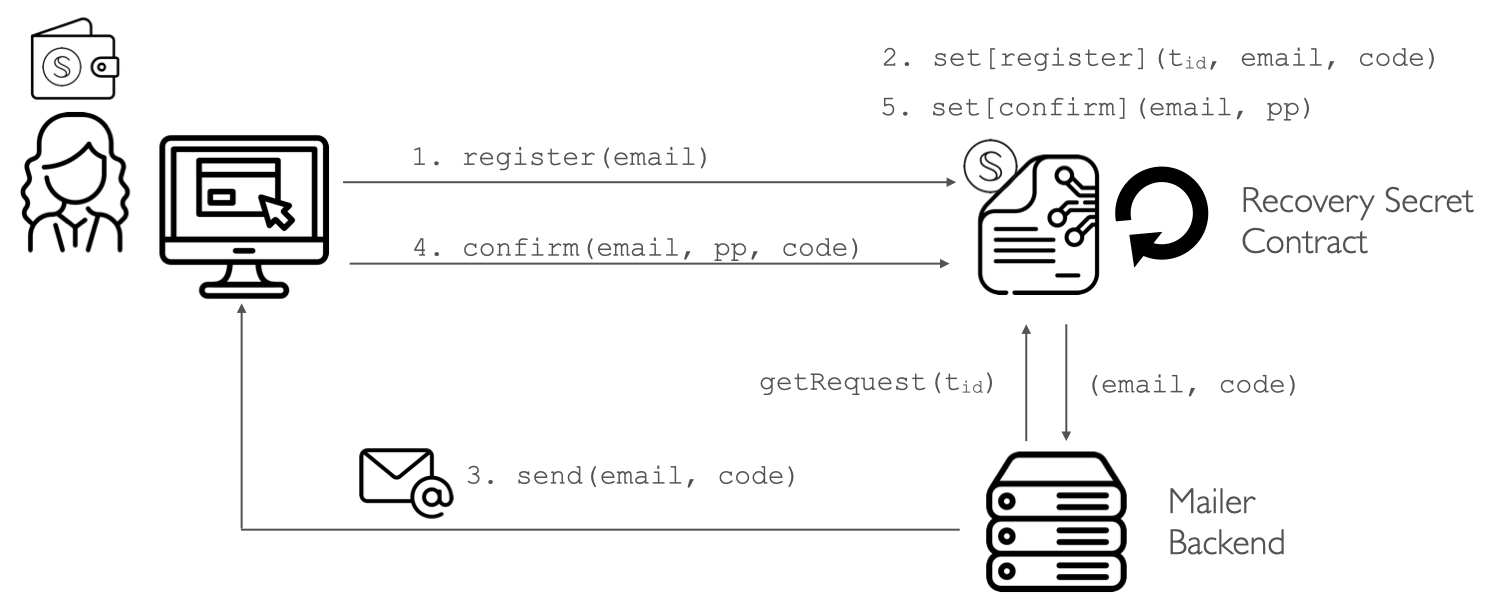
\includegraphics[width=\linewidth]{./media/media-001.png}
  \caption{Iteration 1 - Backup}
  \label{it1:backup}
\end{figure}

\begin{enumerate} 
\item {\bf Request} - Alice enters her $email$ and, after pressing the submit button, a script running inside the webpage sends a transaction {\bf $\ms{register}(email)$} to the Secret Network using a throwaway Secret account that Alice has just provisioned. 
\item {\bf Registration} - The Secret Recovery Contract generates a random confirmation code and stores the record $(t_{id}, email, code)$ in the {\tt register} dataset. 
\item {\bf Emailing} - Once the request transaction has been validated, an event handler is triggered on the Mailer Backend that queries the Recovery Secret Contract for the email and confirmation code associated with the transaction id. Thus, the Mailer Backend sends the confirmation code to Alice by email. 
\item {\bf Confirmation} - Now Alice sees a webpage that asks her to enter the confirmation code sent by email and her passphrase $pp$. She opens her email and copies'n paste the confirmation code into her browser. After pressing the submit button, a script running inside the webpage sends a transaction $\ms{confirm}(email, pp, code)$ to the Recovery Secret Contract. 
\item {\bf Recording} - The Secret Recovery Contract verifies the verification and stores the record $(email, pp)$ in the {\tt confirm} dataset. 
\end{enumerate}

\paragraph{Recovery}

During recovery (see figure~\ref{it1:recovery}), the goal is to verify Alice's email address to eventually send her passphrase back. 

% To do so, Alice needs to create yet another throwaway Secret account to send a transaction to the Recovery Smart Contract. Indeed, it cannot require Alice to use the same Secret account that she used for the backup. If Alice needs to recover a passphrase, she probably no longer have access to it anyway.

\begin{figure}[h!]
  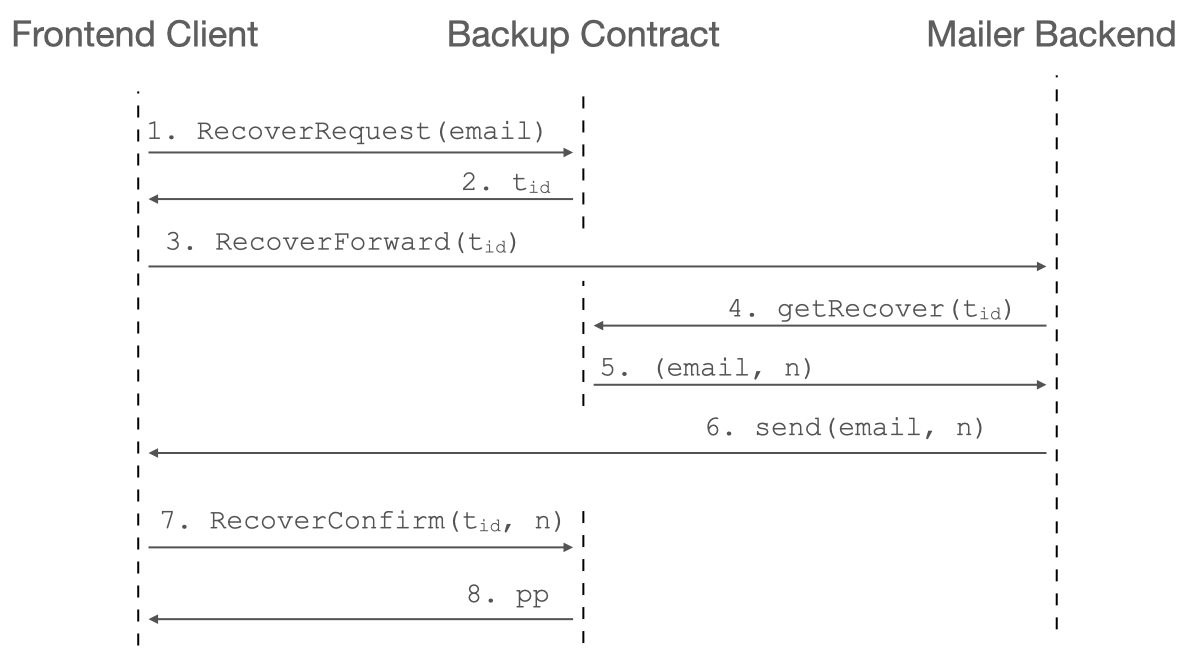
\includegraphics[width=\linewidth]{./media/media-002.png}
  \caption{Iteration 1 - Recovery}
  \label{it1:recovery}
\end{figure}

\begin{enumerate}
\item {\bf Request} - Alice enters her $email$ and, after pressing the submit button, a script running inside the webpage sends a transaction {\bf $\ms{recover}(email)$} to the Recovery Secret Contract to the Secret Network using a throwaway Secret account that Alice has just provisioned. 
\item {\bf Registration} - The Secret Recovery Contract generates a random verification code and stores the record $(t_{id}, email, code)$ in the {\tt recover} dataset. 
\item {\bf Emailing} - Once the request transaction has been validated, an event handler is triggered on the Mailer Backend that queries the Recovery Secret Contract for the email and verification code associated with the transaction id. Thus, the Mailer Backend sends the verification code to Alice by email. 
\item {\bf Verification} - Now, Alice sees a webpage that asks her to enter the verification code sent by email. She opens her email and copies'n paste that verification code into her browser. After pressing the submit button, a script running inside the page sends a query $\ms{verify}(email, code)$ to the Recovery Secret Contract. 
\item {\bf Response} - The Secret Recovery Contract verifies the verification code, retrieves the corresponding record from the {\tt recover} dataset and returns the passphrase.
\end{enumerate}

\subsection{Security Analysis}

Although, this first iteration captures the user experience that we want, it is unfortunately not satisfactory in terms of security. There are three single points of failure: 1) Alice's account, 2) the Mailer Backend and 3) the Secret Recovery Contract. \\

What if Alice's account is hacked? As explained earlier, it is recommended that Alice uses a throwaway Secret account when registering a passphrase. As soon as the passphrase has been recorded, she can forget about this account since she will not need it to recover her passphrase. However, what if the account's private key is leaked somehow? It would be bad since the attacker with this key could look into the transaction history and get the passphrase. \\

What if the Mailer Backend is hacked? Let us consider the two phases: backup and recovery. During the backup phase, the attacker could use the confirmation code to upload an arbitrary passphrase for Alice. This is a problem if Alice recovers what she believes is her original passphrase but is in fact the passphrase to an account that the attacker can access as well. Then, any new asset Alice puts in this account from now on can be stolen by the attacker. During recovery phase it is even worst since the attacker could use the verification code to query the Recovery Secret Contract directly and get the passphrase back. \\

What if the Recovery Secret Contract is hacked? This is by far the biggest threat here since the attacker will have access to all users' passphrases.  \\

Indeed, all of these security threats are not acceptable and we are going to address all of these issues by hardening our protocol in the next iteration. 

\section{Iteration  2: Security Hardening}
\label{iteration2}

As discussed earlier, we should not store all users' passphrases in the same Secret contract in case that contract gets breached. Actually, it would be safer to store each passphrase in its own contract and have those contracts be owned by different accounts. So, for this second iteration, let us try a different approach. Let us have Alice creating a throwaway Secret account to mint a Secret NFT embedding the passphrase as a secret metadata. Then, she sends that NFT to her friend Charlie as a way to backup her passphrase. When the doomsday comes, she could recover her passphrase by asking Charlie to send her NFT back. Indeed, this approach is not secure since Charlie could access the passphrase as soon as he owns the NFT. A solution to that is to have Alice encrypting her passphrase when minting the NFT so that Charlie cannot decrypt without the key. However, we have another problem now, where to store the key when Alice needs it to recover her passphrase? We could actually adopt the same approach as describe in iteration 1. Instead of storing all passphrases in the Recovery Smart Contract, we could store all users' encryption keys. But, did not we say that this was insecure? It is more secure actually. While it is true that all the keys would be exposed if the contract is breached, however, those keys are now worthless if the attacker is not able to locate and regain those NFTs one by one to extract each passphrase. Our system is more secure since breaking those passphrases is now lot harder for the attacker. \\

There were two other problems we identified in iteration 1 that do not go away with our new NFT approach. First, if an attacker could hacks into Alice's backup account, he could recover the key sent to the Recovery Secret Contract. Secondly, if an attacker could hacks into the mailer backup, he could also recover the key by getting the verification code. In this approach we fix those two problems by implementing the Diffie-Hellman Key Exchange key protocol on the Secret blockchain. The goal is to have Alice's account and the Recover Secret Contract negotiate a key without exchanging it explicitly during the backup phase.

\subsection{The Diffie-Hellman Key Exchange Protocol}

The {\em Diffie–Hellman Key Exchange Protocol} is a cryptography protocol that allows two parties, usually named Alice and Bob, that have no prior knowledge of each other, to securely agree on a shared key over an insecure channel. That channel is considered as insecure because we assume that an attacker, usually named Eve, can eavesdrop the communication and read all messages send back and forth between Alice and Bob. \\

The algorithm relies on modular arithmetics but let us abstract the mathematical details by simply saying that Alice generates two numbers: one ``secret'' $sec_A$ that Alice will keep and another one ``public'' $pub_A$ that Alice can send to Bob over the insecure channel. When Bob receives Alice's public number, he will also generates its own pair $(sec_B, pub_b)$ and send his public number back to Alice. Once the public numbers have been exchanged, Alice and Bob can generate the same shared secret value $s$. Alice computes $s=\ms{ECDH}(sec_A, pub_A, pub_B)$ and Bob computes the same shared secret value $s=\ms{ECDH}(sec_B, pub_B, pub_A)$. The security of the protocol reside in the fact that it is impossible for Eve to compute that secret value $s$ even if she knows $pub_A$ and $pub_B$ because she does not know either $sec_A$ or $sec_B$. \\

In practice, this shared secret value is usually not used as a cryptographic key directly. Instead, that shared value is given as input of a key derivation function such as $\ms{PBFK2}$ that will generate the same cryptographic key based based on the secret value. 

\subsection{The Protocol}

Moreover, we are adding two additional features to our NFT-based Mnemonic Backup System. First, Alice can now backup several passphrases and still recover each of them with the same email. To do so, she will attach a unique id with each NFT during backup and ask the Recovery Smart Contract for that specific id when she needs to recover the associated key. Secondly, Alice has now a limited time to enter her confirmation code during backup or validation code during recovery. this time limit is calculated based on the number of blocks that have been validated since Alice has made her original request to the Secret Recovery Contract. \\

All of those new features are detailed in the new version of the protocol shown in figures \ref{it2:backup} and \ref{it2:recovery}.

\paragraph{Backup}

\begin{figure}[h!]
  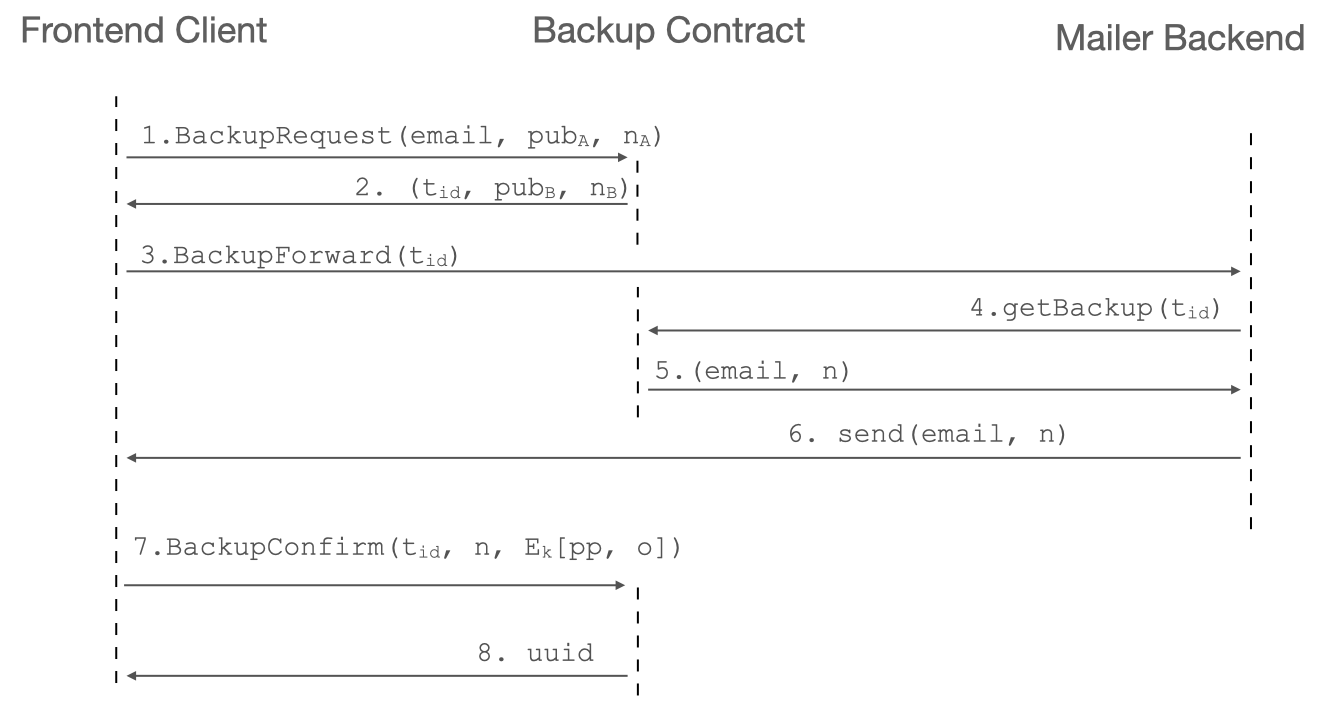
\includegraphics[width=\linewidth]{./media/media-003.png}
  \caption{Iteration 2 - Backup}
  \label{it2:backup}
\end{figure}

\begin{enumerate} 
\item {\bf Request} - Alice enters her $email$, her passphrase $m$, an $id$ for her passphrase. After pressing the submit button, a script running inside the webpage generates an ECDH private and public key pair $(sec_A, pub_A)$, a nonce $n_A$ and sends the transaction $\tx{request}{t_{id}, b_{id}}{email, id, pub_A, n_A}$ to the Secret Network using the throwaway Secret account that Alice has just provisioned. 
\item {\bf Registration} - The Secret Recovery Contract generates a new ECDH private and public key pair $(sec_B, pub_B)$ and a nonce $n_B$. It calculates the ECDH secret $s=\ms{ECDH}(sec_B, pub_B, pub_A)$ and derives the 128-bit AES symmetric key $k$ using the standard password-based key derivation function $\ms{PBFK2}$ and the concatenation of $n_A$ and $n_B$ as a salt $k=\ms{PBKDF2}(s, n_A || n_B)$. Finally, the contract stores the record $(email, id, t_{id}, b_{id}, pub_B, n_B)$ in the {\tt register} dataset.
\item {\bf Emailing} - Once the request transaction has been validated, an event handler is triggered on the Mailer Backend that queries the Recovery Secret Contract $\qry{info}{t_id}$. The Secret Recovery Contract checks that the query comes from the Mailer Backend address, retrieves the record from the {\tt register} dataset and checks that the query has not expire based on the initial block id $b_{id}$ and the current block id on the Secret Network. If not, it returns the $email$, the public key pair $pub_B$ and the nonce $n_B$. Finally, the mailer daemon sends an email to Alice with the confirmation code $(pub_B, n_B)$. 
\item {\bf Confirmation} - Now Alice sees a webpage that asks her to enter the confirmation code sent by email and her passphrase $pp$. She opens her email and copies'n paste the confirmation code into her browser. After pressing the submit button, a script running inside the webpage calculates the ECDH secret $s=\ms{ECDH}(sec_A, pub_A, pub_B)$ and derives the 128-bit AES symmetric key $k$ using $\ms{PBFK2}$ and the concatenation of $n_A$ and $n_B$ as a salt $k=\ms{PBKDF2}(s, n_A || n_B)$. Then, it calculates a hash-based message authentication code (abbreviated HMAC) using the key $k$ and the concatenation of the email and id $h=\ms{HMAC}(k, email || id)$. Finally, the script sends the transaction $\tx{confirm}{t_{id}', b_{id}'}{email, id, h}$ to the Secret Network. 
\item {\bf Recording} - The Secret Recovery Contract checks that the query has not expire based on the initial block id $b_{id}$ and the current block id on the Secret Network. Then, it calculates the HMAC of the concatenation of the email and id using the key $h=\ms{HMAC}(k, email || id)$ and checks that this hash is strictly equal to the hash $h$ in the request. Finally, the contract stores the tuple $(email, id, k)$ in the {\tt confirm} dataset.
\item {\bf NFT minting} - The client-side script can now encrypt (using AES in GCM mode) the passphrase $m$ with the key $k$ to obtain the ciphertext $c=E_{\ms{AES}}(k, m)$. It mints a Secret NFT with the concatenation of the id and the ciphertext as private metada.  
\end{enumerate}

Once the protocol is completed, Alice can transfer the NFT to Charlie. 

\paragraph{Recovery}

\begin{figure}[h!]
  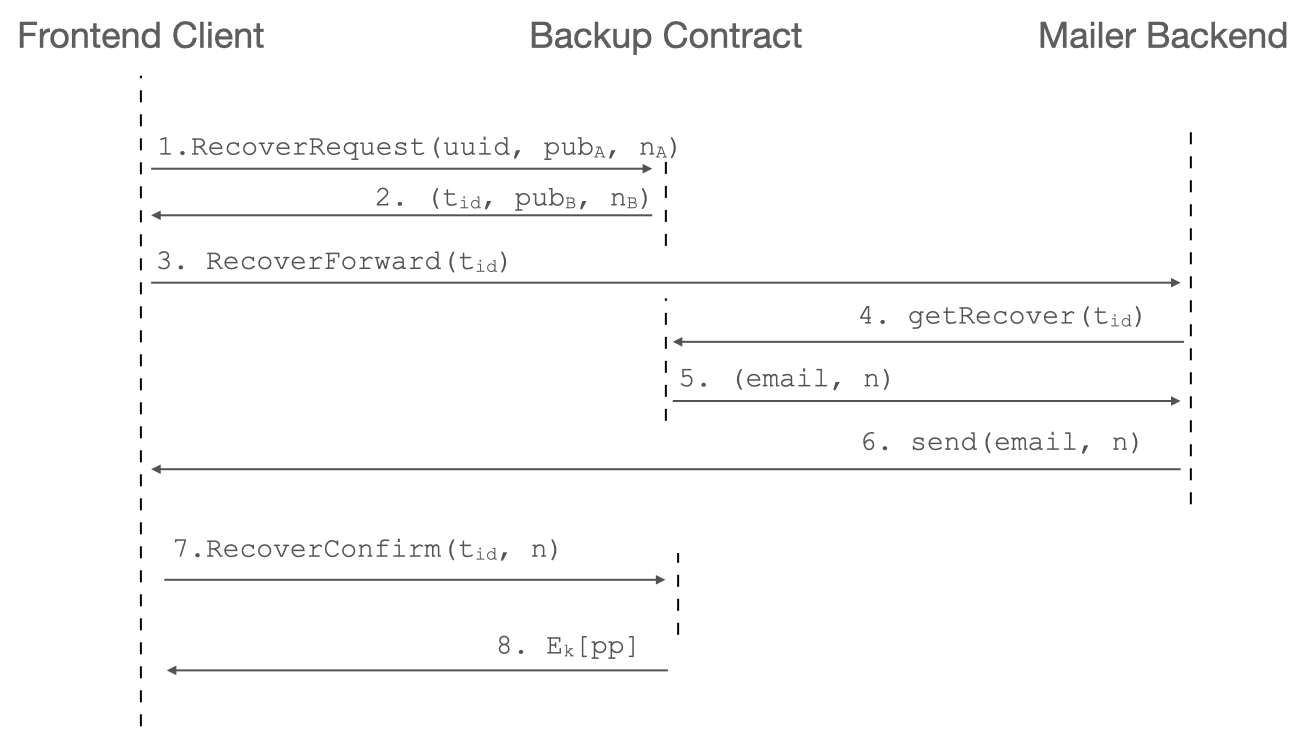
\includegraphics[width=\linewidth]{./media/media-004.png}
  \caption{Iteration 2 - Recovery}
  \label{it2:recovery}
\end{figure}

\begin{enumerate}
\item {\bf Request} - Alice creates a new Secret Wallet and asks her friend to send the NFT back. Then, she goes to the recovery page that asks her to select the NFT. A script running inside the webpage extracts the $id$ and the ciphertext from the NFT. Finally, it generates a nonce $n_A$ and sends the transaction $\tx{request}{t_{id}, b_{id}}{email, id, pub_A, n_A}$ to the Secret Network. 
\item {\bf Registration} - The Secret Recovery Contract retrieves the record from the {\tt confirm} dataset using the email and id from the transaction. Then, it generates a nonce $n_B$ and stores the record $(email, id, t_{id}, b_{id}, n_B)$ in the {\tt register} dataset.
\item {\bf Emailing} - Once the request transaction has been validated, an event handler is triggered on the Mailer Backend that queries the Recovery Secret Contract for the email and verification code associated with the transaction id. The Secret Recovery Contract checks that the query comes the Mailer Backend and retrieves the record from the {\tt register} dataset and checks that the query has not expire based on the initial block id $b_{id}$ and the current block id on the Secret Network. Then, it returns the $email$ and the nonce $n_B$. Finally, the mailer daemon sends an email to Alice with the verification code $n_B$. 
\item {\bf Verification} - Now, Alice sees a webpage that asks her to enter the verification code sent by email. She opens her email and copies'n paste that verification code into her browser. After pressing the submit button, a script running inside the page calculates the hash of the concatenation of the two nonces $h=\ms{H_{\ms{SHA512}}}(n_A || n_B)$. The script sends a query $\tx{verify}{t_{id}', b_{id}'}{email, id, h}$ to the Secret Network. 
\item {\bf Response} - The Secret Recovery Contract checks that the query has not expire based on the initial block id $b_{id}$ and the current block id on the Secret Network. Then, it calculates the hash of the concatenation of the two nonces $h=\ms{H_{\ms{SHA512}}}(n_A || n_B)$ and checks that this hash is strictly equal to the hash $h$ in the request. Finally, it returns the key $k$ back to the client
\item {\bf Passphrase Decryption} - After receiving the key back, the client-side script can now decrypt the ciphertext $c$ to obtain the passphrase $m=D_{\ms{AES}}(k, c)$. 
\end{enumerate}

Once the protocol is completed, Alice sees her passphrase on the webpage.

\subsection{Security Analysis}

This second iteration of our Mnemonic Backup System is more secured. Let us discuss each entity in our architecture. \\

What if Alice's account is hacked? As explained earlier, it is recommended that Alice uses a throwaway Secret account when registering a passphrase. However, if the account's private key was leaked, an attacker could know to which address the NFT has been transfered but could not retrieve the encryption key with the information recorded in the different transactions. \\

What if the Mailer Backend is hacked? Let us consider the two phases: backup and recovery. During the backup phase, the attacker could not use the confirmation to upload an arbitrary key since the attacker does not know the client's id and ECDH secret. During the recovery phase, the attacker could retrieve the key but without locating and getting each Secret NFT back, the attacker will not be able to get the passphrase. \\

What if the Recovery Secret Contract is hacked? The attacker would be able to get all of the encryption keys but, again, without locating and getting each Secret NFT back, the attacker will not be able to get the passphrase. The fact that the encrypted passphrase is embedded in a Secret NFT separated from the Recovery Secret Contract is the most important security features that makes our system resilient to attacks. \\

However, having a friend holding the Secret NFT introduces another problem: what if that friend does not or cannot return the NFT back? The passphrase would be locked forever. We are improving this availability issue in our next and final iteration. 

\section{Iteration 3: Improving Availability}
\label{iteration3}

Having a unique friend holding Alice's NFT can be a problem if that friend does not or cannot return it to her. A naive solution would be to duplicate the same NFT and send it to multiple friends. This solution is not ok but not ideal in terms of security since we are extending the attack surface. The attacker can now target multiple people to regain one of these NFTs. In this third and last iteration, we adress the availability problem while preserving the security of our system by using the Shamir's Secret Sharing scheme. 

\subsection{The Shamir's Secret Sharing Scheme}

Shamir's Secret Sharing scheme is a cryptography protocol usually used for splitting a secret into into multiple parts, called shares, which individually do not give any information away about that secret. To recover that secret, not all shares are needed but a minimun of shares called {\em ``the threshold''}. On one hand, this is ideal from the usability perspective since the user does not have to collect all the shares back but only the minimum threshold required. On the other hand, this is perfect from the security perpective since any attacker who discovers any number of shares less than the threshold will not be able to break the secret. \\

\subsection{The Protocol}

\begin{figure}[h!]
  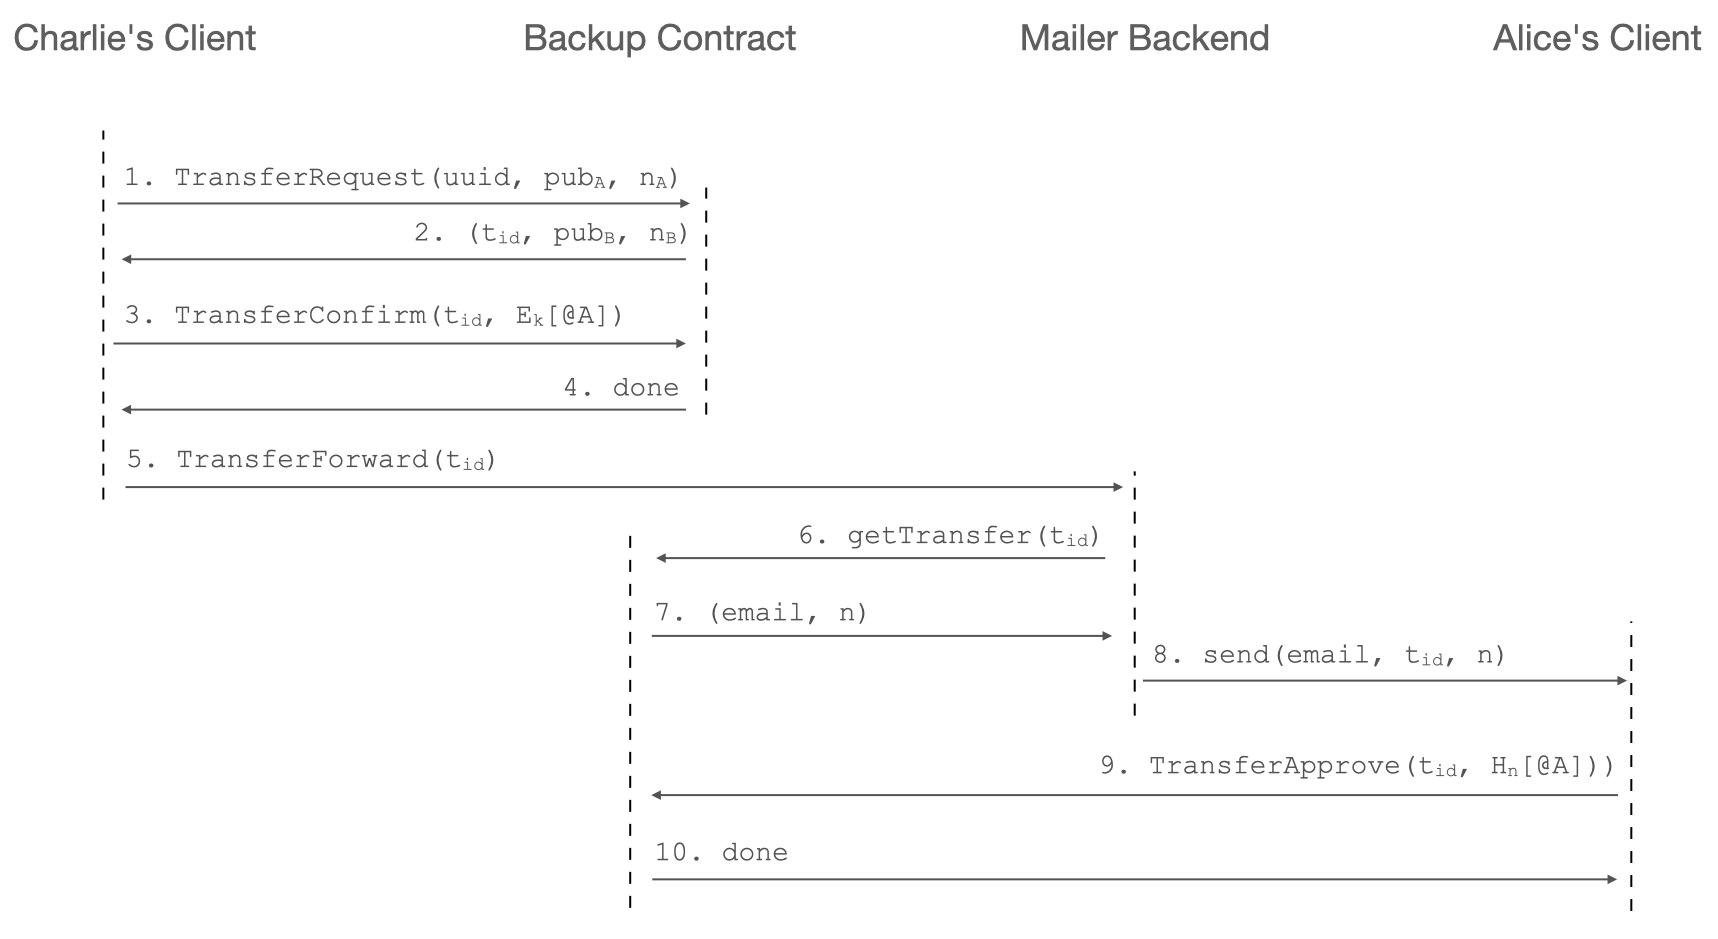
\includegraphics[width=\linewidth]{./media/media-005.png}
  \caption{Iteration 3 - Shamir's Secret Sharing NFTs}
  \label{it3:backup}
\end{figure}

{\bf For the backup}, Alice needs to specify the number of shares $i$ she wants to generates and the minimum number of shares $j$ needed to retrieve the passphrase (threshold value). Once, the encryption key has been fully registered in the contract, the script encrypts the passphrase, concatenates the id and the ciphertext to generate the $i$ shares using the SSS algorithm: $(s_1,\cdots,s_i)=E_{\ms{SSS}}(id||c, i, j)$. Finally, the script mints the $i$ Secret NFTs on the Secret Network. Once the protocol is completed, Alice can now transfer the NFTs to her accointances. \\

{\bf For the recovery}, Alice creates a new Secret Wallet and asks all of her friends to send their NFTs back. Once she has at least $j$ of those NFTs on her wallet, she goes to the recovery page that asks her to select the NFTs. Then, the script in the webpage collects the shares and extracts the $id$ and the ciphertext from the NFTs $id||c = D_{\ms{SSS}}(s_1,\cdots,s_j)$. Then, the protocol continues like in the previous iteration. 

\section{Value Capture for Secret Network Ecosystem}

This backup system will demonstrate that the Secret Network privacy model is adequate to keep sensitive information confidential relying on two important features of Secret NFTs: secret metada and private ownership \\ 

Why implementing our backup system on Secret Network rather than Ethereum? Is it because Ethereum-based NFTs do not have secret metadata? Not really since we could have created a password protected version of the share and hid it inside a public NFT image using Steganography \cite{Steganography}. The real problem is that if an attacker knows that an NFT contains a share to recover a mnemonic phrase, he or she will be able to locate all others NFTs that contains the other shares easily since ownership is public on Ethereum. The fact that Secret NFTs protects the ownership is the key feature that makes our backup system secured. 

\section{Conclusion}

In this paper, we propose a Decentralized Mnemonic Backup system that anyone can use to give custody to any blockchain passphrase to the Secret Network \cite{SecretNetwork} and recover it using a simple email. The idea is to encrypt the passphrase and split it into multiple Secret NFTs using the Shamir's Secret Sharing cryptographic protocol. The encryption key is saved in a Secret smart contract. This key is never recorded in any transaction. Instead, it is generated using the Diffie-Hellman Key Exchange Protocol that is similarly used in well known protocols such as TLS and Signal. \\

The key recovering system can be used outside of our Mnemonic Backup system. It can be used for more advanced cryptographic protocols that involve storing and managing secret keys on chain with the option of recovering it using an email. For instance, this can be used to encrypt files on IPFS and manage the access using a Secret Contract that would hold custody of the encryption key. Such an approach has been proposed by {\em DataVault} in \cite{DataVault}. However, the {\em DataVault} white paper does not provide any details regarding how the encryption key handle on the Secret Network. Our system could be used to safely generate and manage the encryption key on the Secret Network and possibly have an email backup solution if such feature is desired.  

\begin{thebibliography}{9}

\bibitem{LostPasswords} Lost Passwords Lock Millionaires Out of Their Bitcoin Fortunes, \url{https://www.nytimes.com/2021/01/12/technology/bitcoin-passwords-wallets-fortunes.html}

\bibitem{BIP39} Mnemonic Generation (BIP39) Simply Explained, \url{https://medium.com/coinmonks/mnemonic-generation-bip39-simply-explained-e9ac18db9477}

\bibitem{MetamaskFAQ} Metamask FAQ page, \url{https://metamask.io/faqs/}

\bibitem{1password} 1password, \url{https://support.1password.com/forgot-account-password/}

\bibitem{SecretNetwork} Secret Network: A Privacy-Preserving Secret Contract \& Decentralized Application Platform, \url{https://scrt.network/graypaper}

\bibitem{Steganography} Steganography, \url{https://en.wikipedia.org/wiki/Steganography}

\bibitem{DataVault} DataVault — A Modular Encrypted Data Paywall and Storage Access Protocol \url{https://data-vault.medium.com/datavault-a-modular-encrypted-data-paywall-and-storage-access-protocol-773a60cfbabb}

\end{thebibliography}

\end{document}
